\section{Foundations}
\subsection{Derivation of EOM of many body system}
Hamiltonian of single atom dispersively coupled to single cavity mode by a running-wave laser drive 
\begin{equation}
	\hat{H}_{SP} = \frac{\hat{p}^2}{2M}- \hbar \omega_z \hat{F}_z + \hbar q \hat{F}^2_z + \hbar \omega_c \hat{a}^\dag \hat{a}-i \frac{\alpha_\nu}{2F}\left [ \bm{\hat{E}}^{(+)} \cross \bm{\hat{E}}^{(-)} \right ] \cdot \bm{\hat{F}} .
\end{equation}
Operator $\hat{a}$ creates photon in z-polarized cavity mode of frequency $\omega_c$. Second and third term are Zeeman splittings. $\bm{\hat{F}}$ is spin operator.
\begin{figure}[h!]
	\centering
	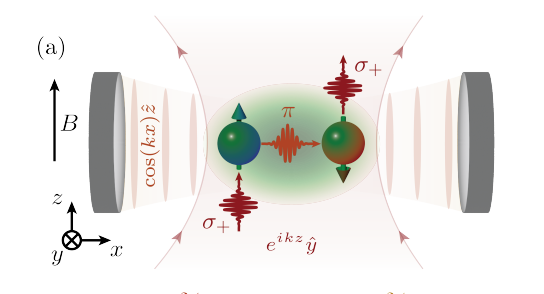
\includegraphics[width=1\linewidth]{Images/scetch_pair_production.png}
	\caption{Pair production}
	\label{fig:scetch_pair_production}
\end{figure}
\\ \break
Second quantization 
\\ \break
Spinor field operator \text{RHS "5-mode-expansion" doesnt contain second summand}
\begin{equation}
	\hat{\Psi} (\bm{x}) = \left (
	\begin{matrix}
		\frac{k}{\sqrt{2}\pi} \cos(kx) ( e^{ikz}\hat{c}_{+k,+1} + e^{-ikz} \hat{c}_{-k,+1})
		\\
		\frac{k}{2 \pi}\hat{c}_{0,0} + \frac{\sqrt{2}k}{\sqrt{3}\pi} \cos^2(kx)\hat{c}_{\pm2k_x,0}
		\\
		\frac{k}{\sqrt{2}\pi} \cos(kx) ( e^{-ikz}\hat{c}_{-k,-1} + e^{ikz} \hat{c}_{+k,-1})
	\end{matrix} \right)
	= \left (
	\begin{matrix}
		\hat{c}_{+1,+k} \psi_{+1,+k} + \hat{c}_{+1,-k} \psi_{+1,-k}
		\\
		\hat{c}_{0,0}\psi_{0,0} 
		\\
		\hat{c}_{-1,k} \psi_{-1,+k} + \hat{c}_{-1,-k}\psi_{-1,-k}
	\end{matrix}
	\right)
\end{equation}
Where the respective functions have to be normed
\begin{equation}
	\int_{\frac{-\pi}{k}}^{\frac{\pi}{k}}  \psi^*_{+1,+k} \psi_{+1,+k} dz dx = 1
\end{equation}(c.f. 2010 Dicke paper)
\begin{equation}
	\Psi = \left( \begin{matrix}
		\Psi_{+1}
		\\
		\Psi_0
		\\
		\Psi_{-1}
	\end{matrix}\right)
\end{equation}
Next we find an effective many body hamiltonian.
\begin{equation}
	H_{SP} = H_L + H_{AT} + H_{INT}
\end{equation}
Where $H_{AT}$ contains $F_z$ and $H_{INT}$ contains $F_+, F_-$.
\begin{equation}
	H_{MB} = H_L + \int \hat{\Psi}^\dag(\hat{x}) ( H_{AT} + H_{INT}) \hat{\Psi}(\hat{x}) \hat{dx}
\end{equation}

e.g. 
\begin{equation}
	F_z = \left( 
	\begin{matrix}
		+1 && 0 && 0
		\\
		0 && 0 && 0 
		\\ 
		0 && 0 && -1
	\end{matrix}
	\right) 
\end{equation}
\begin{equation}
	F_+ =\sqrt{2} \left( 
	\begin{matrix}
		0 && 1 && 0
		\\
		0 && 0 && 1 
		\\ 
		0 && 0 && 0
	\end{matrix}
	\right) 
\end{equation}
This calculation is done in Rodrigos "Full derivation Hamiltonian" handwritten pdf. We do adiabatic elimination with effective operators and apply the rotating wave approximation. 
We obtain the effective many-body Hamiltonian
\begin{equation}\label{eq:fou_effective_many_body_hamiltonian}
	H = H_0 + H_+ + H_-
\end{equation}
with e.g.
\begin{equation}
	H_+ = \hbar \chi_+ (2 \hat{c}^\dag_{-k,-1} \hat{c}^\dag_{+k,+1}\hat{c}_0 \hat{c}_0+ \hat{c}^\dag_0 \hat{c}_{+k,+1}\hat{c}^\dag_{+k,+1}\hat{c}_0 + \hat{c}^\dag_{-k,-1}\hat{c}_0\hat{c}_0^\dag \hat{c}_{-k,-1} + h.c.)
\end{equation}
\subsection{Further info to experiment: (rodrigo thesis p.103)}
drive is operated in limit of large two-poton  detunings
\begin{equation}
	|\delta_\pm| \gg \kappa
\end{equation}
\begin{equation}
	\delta_\pm = \delta_c \pm \omega_z = (\omega_d \pm \omega_z) - \omega_c
\end{equation}
We absorb drive photon, and go from 
\begin{equation}
	\ket{0}_0 \rightarrow \ket{+k}_+1
\end{equation}
thus we need a energy conserving cavity photon with freq $\approx \omega_d - \omega_z$. (or $+\omega_z$?) Here we can still ignore the kinetic energy $\sim k$ of the atom since this energy is much smaller than $\kappa$.
\\ 
Parametric amplification of pair production
\\
look at \ref{eq:fou_effective_many_body_hamiltonian} + assume mode $\ket{0}_0$ undepleted throughout the dynamics i.e. occupied by N atoms. set $\hat{c}_0$ = $\sqrt{N}$ and obtain
\begin{equation}
	\hat{H}_{eff} = \hat{H}^+_{eff} + \hat{H}^-_{eff}
\end{equation}
with 
\begin{equation}
	\hat{H}^\pm_{eff} = \hbar (\omega_0 + 4 N \chi_\pm)(\hat{K}_{z,\pm}-1/2) + 4 \hbar N \chi_\pm \hat{K}_{x,\pm}
\end{equation}
Look at linear equations of motion
\begin{equation}\label{eq:fou_time_development_linear_K}
	\dt{}\left( 
	\begin{matrix}
		\hat{K}_{x,\pm}
		\\
		....y
		\\
		...z
	\end{matrix}\right) = \bm{M}_\pm 
	\left( \begin{matrix}
	\hat{K}_{x,\pm}
	\\
	....y
	\\
	...z
	\end{matrix}\right)	
\end{equation}
with three non-degenerate complex eigenvalues
\begin{align}
	\lambda_{1,\pm} = 0 
	\\
	\lambda_{2,\pm} = \sqrt{-\omega_0(\omega_0 + 8 N \chi_\pm)} \eqcolon + \lambda_\pm
	\\
	\lambda_{3,\pm} = - \sqrt{- \omega_0 (\omega_0+8N \chi_\pm)}
\end{align}
We also have
\begin{equation}\label{eq:fou_time_development_particle_number}
	\langle N_{p,\pm} \rangle = \frac{1}{2} (\langle c_{1,\pm}^\dag c_{1,\pm} \rangle + \langle c_{-1,\mp}^\dag c_{-1,\mp}\rangle ) \approx \langle K_{z,\pm} \rangle - \frac{1}{2} \approx A\cosh(\lambda_\pm t) + \text(const)
\end{equation}
To conclude: we see that we have eigenvectors of M. Those are perpendicular, since the eigenvalues are different. The time development of those is given by \ref{eq:fou_time_development_linear_K}. Thus, its either phase oszillation for a complex eigenvalue or exponential growth for a real eigenvalue. \ref{eq:fou_time_development_particle_number} looks at the expectation value of the occupation of the modes that are not $\ket{0}_0$ (occupation of pairs). we see that the time development of those depends on $ \langle K_{z,\pm} \rangle$, therefore on the eigenvectors of M, therefore on the eigenvalues of M. We see, that for a real $\lambda_\pm$ the occuopation of those modes get macroscopic. So we say that for a critical coupling a second order phase transition occurs (lambda get real) featuring pairs. this fast change of coupling is called quench (faster that any period of oscillations happening in system e.g. $1/\omega_0$). 
\\
Note: if the number of pairs gets high, the undepleted approximation doesnt hold anymore. thus this equations can just predict the inital growth of pairs. (later there is saturation)
\\
quench: the system jumps from one set of eigenstates to another set of eigenstates. before system was in single eigenstate, after quench it is superposition of different eigenstates $\rightarrow$ oscillation of those. this cant be expressed analytically, thus calculations are done numerically. 
\begin{figure}[h!]
	\centering
	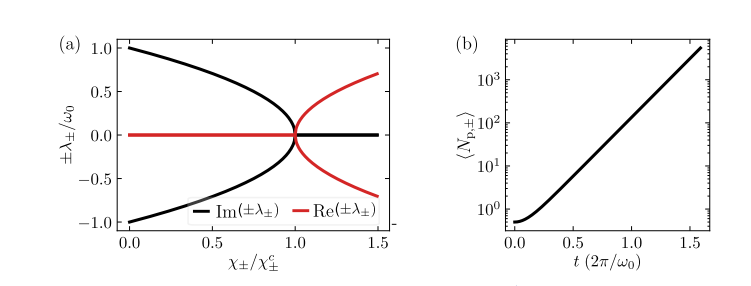
\includegraphics[width=1\linewidth]{Images/scetch_quench_parametric_amplification.png}
	\caption{Parametric amplification}
	\label{fig:scetch_quench_parametric_amplification}
\end{figure}
